\documentclass[a4paper,11pt,fleqn]{article}
\usepackage[utf8x]{inputenc}
\usepackage{ucs}
\usepackage[T2A,OT4]{fontenc}
\usepackage[a4paper,top=2.5cm,bottom=2.5cm,left=2.5cm,right=2.5cm]{geometry}
\usepackage[MeX]{polski}
\usepackage{titling}

%\usepackage{bold-extra}

\usepackage{amssymb}
\usepackage{amsmath}
%\usepackage{amsthm}
%\usepackage{gensymb}

%\usepackage{wrapfig}
\usepackage{graphicx}
%\usepackage{lipsum}
%\usepackage{epstopdf}
\usepackage{caption}
%\usepackage{subcaption}
%\usepackage{adjustbox}
%\usepackage{dcolumn}
%\newcolumntype{d}[1]{D{,}{,}{#1}}


\usepackage{xcolor}
%\colorlet{zaglowek}{blue!10}
\usepackage{indentfirst}
\usepackage{fancyhdr}
\usepackage{lastpage}
%\setlength{\headheight}{13.6pt}
\usepackage{listings}
%\usepackage{slashbox}

\author{Jakub Kasznia \and Paulina Wr\'obel}
%\title{Modelowanie i symulacja wybranych struktur modulator\'ow Sigma--Delta}
\title{Modelowanie i analiza system\'ow -- dice game}
\date{09.03.2016r.}

\makeatletter
\let\mytitle\@title
\makeatother

\usepackage[pdftex,
            pdfauthor={\theauthor},
            pdftitle={\thetitle\ --- \theauthor},
            pdfsubject={Sprawozdanie},
            pdfkeywords={VHDL},
            pdfproducer={Latex},
            pdfcreator={pdflatex},
            hidelinks]{hyperref}

%\fancyhead{} 
%\fancyfoot{} 
%\fancyfoot[C]{Strona \thepage \ z \pageref*{LastPage}} 
%\renewcommand{\headrulewidth}{0pt} 
%\renewcommand{\footrulewidth}{0.4pt}

\fancyhf{}
\fancyhead[R]{\textit{\mytitle}}
\fancyhead[L]{\textit{\theauthor}}
\fancyfoot[C]{\thepage}%comment for oneside
%\fancyfoot[R]{\thepage}%and also onepage
\renewcommand{\headrulewidth}{0.4pt} 
\renewcommand{\footrulewidth}{0pt}

\lstdefinelanguage{Modelsim}{
  morekeywords={
    force,run,all,vcom,vsim,add,wave
  }%,
  %morecomment=[l]#
}

\lstdefinestyle{VHDLStyle}{
language=VHDL,
flexiblecolumns=true,
frame=l,
basicstyle=\ttfamily,
keepspaces=true,
rulecolor=\color{black!40},
%keywordstyle=\color{blue!70!black},
commentstyle=\color{green!50!black},
aboveskip=8pt,
belowskip=10pt,
numbers=left,
numbersep=6pt,
stepnumber=1,
stringstyle=\color{magenta!80!blue},
numberstyle=\small\color{black!45},
inputencoding=utf8x,
extendedchars=\true}

\lstdefinestyle{ModelsimStyle}{
language=Modelsim,
flexiblecolumns=true,
frame=l,
basicstyle=\ttfamily,
keepspaces=true,
rulecolor=\color{black!40},
keywordstyle=\color{blue!70!black},
commentstyle=\color{green!50!black},
aboveskip=8pt,
belowskip=10pt,
numbers=left,
numbersep=6pt,
stepnumber=1,
stringstyle=\color{magenta!80!blue},
numberstyle=\small\color{black!45},
inputencoding=utf8x,
extendedchars=\true}


\begin{document}

\pagestyle{fancy}
\thispagestyle{plain}



\newgeometry{tmargin=2cm, bmargin=2.5cm, lmargin=2.5cm, rmargin=2.5cm} 
%\vspace{-2ex}
\begin{table}[h]
\begin{center}
\noindent
\begin{tabular}{|c|c|c|}\hline
\multicolumn{3}{|c|}{\textsc{\large{sprawozdanie z laboratorium}}}\\\hline
\multicolumn{2}{|l|}{\small{Przedmiot}}&\small{Rok akademicki}\\
\multicolumn{2}{|c|}{\Large{\textbf{Modelowanie i analiza systemów}}}&\textbf{2015/16}\\\hline
\multicolumn{2}{|l|}{\small{Temat ćwiczenia}}&\small{Termin zajęć:}\\
\multicolumn{2}{|c|}{\textbf{\Large{Dice Game}}}&{\textbf{środa}}\\
\multicolumn{2}{|c|}{\textbf{\Large{}}}&{\textbf{12:45--15:00}}\\\hline
\multicolumn{1}{|l|}{\small{Wydział}}&\multicolumn{2}{|l|}{\small{Kierunek, specjalność}}\\
\textbf{Wydział Informatyki}&\multicolumn{2}{|l|}{\textbf{Informatyka, Mikrosystemy Informatyczne}}\\\hline
\multicolumn{1}{|l|}{\small{Semestr}}&\multicolumn{1}{|l|}{\small{Skład grupy}}&\multicolumn{1}{|l|}{\small{Data wykonania}}\\
\textbf{Semestr 1}&\textbf{Jakub Kasznia, Paulina Wróbel}&\textbf{31.05.2016r.}\\\hline
\end{tabular}
\end{center}
\end{table}


\section{Reguły gry}

Celem ćwiczenia jest zaprojektowanie i przetestowanie w zaproponowanym testbench'u modelu gry Dice Game.

\vspace{2ex}

Wejściami do układu są sygnały:
\begin{itemize}
\item \texttt{Reset} -- przycisk inicjujący grę,
\item \texttt{Rb} -- \textit{Roll button} -- przycisk symulujący wyrzut kostek.
\end{itemize}

Wyjściami z układu są sygnały:
\begin{itemize}
\item \texttt{Win} -- dioda sygnalizująca wygraną,
\item \texttt{Lose} -- dioda sygnalizująca przegraną,
\item wyświetlacz pokazujący wyrzucone liczby i ich sumę.
\end{itemize}

Symulacja wyrzutu kostek jest realizowana przez dwa liczniki o różnych częstotliwościach. Poniżej przedstawiono reguły gry. Wygnana i przegrana zależy od numeru iteracji:
\begin{itemize}
\item pierwszy wyrzut kostek:
    \begin{itemize}
    \item wygrana -- wylosowanie sumy 7 lub 11, 
    \item przegrana -- wylosowanie sumy 2, 3 lub 12,
    \item w innych przypadkach można losować jeszcze raz,
    \end{itemize}
\item drugi wyrzut kostek i kolejne:
    \begin{itemize}
    \item wygrana -- wylosowanie takiej samej sumy jak poprzednio, 
    \item przegrana -- wylosowanie sumy 7,
    \item w innych przypadkach można losować jeszcze raz.
    \end{itemize}
\end{itemize}





\newpage
\section{Model bez liczników i sumatora}

\subsection{Struktura układu}

Na rys.~\ref{noSum} przedstawiona jest struktura, na podstawie której napisano kod w VHDL. 


\begin{figure}[h]
\centering
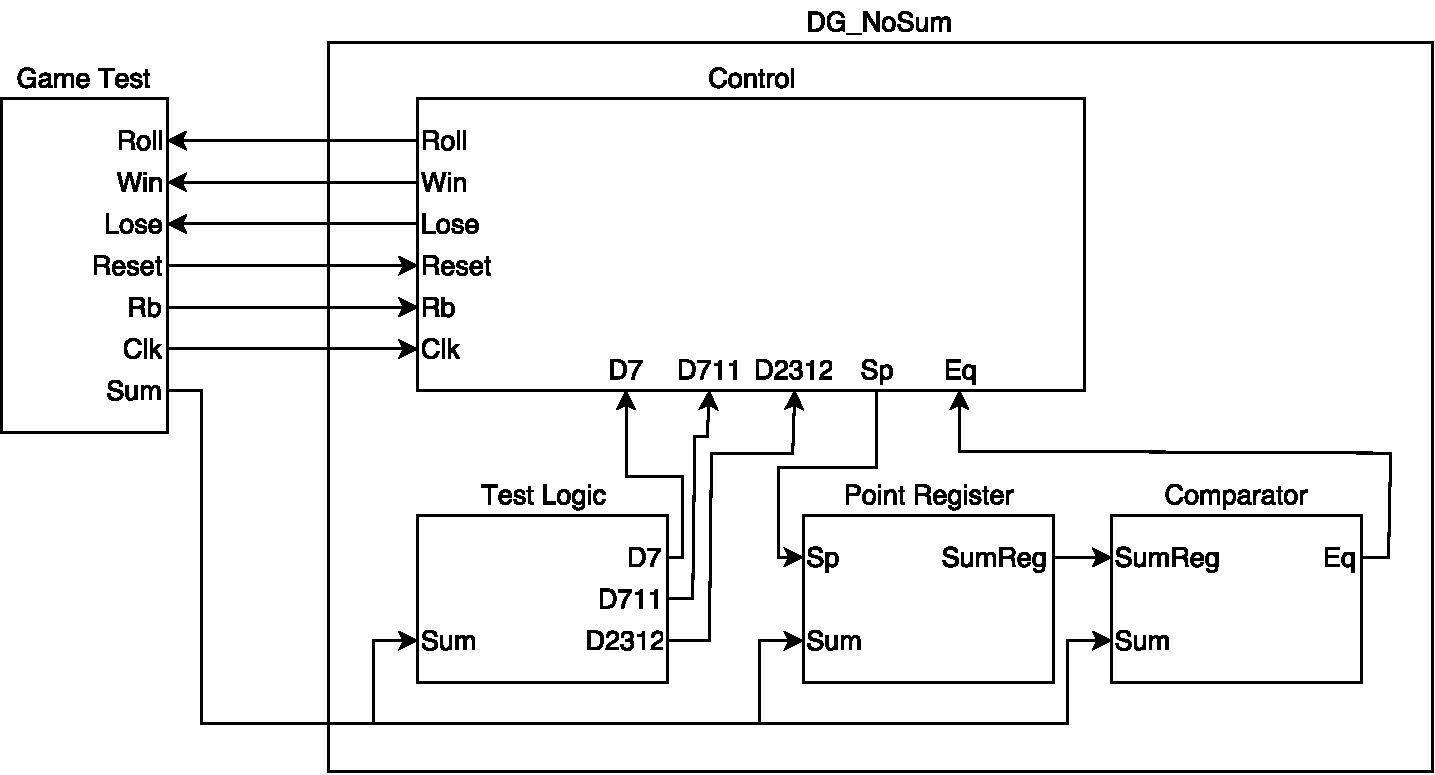
\includegraphics[width=\textwidth]{schematics/noSum.pdf}
\caption{Struktura układu bez liczników i sumatora}
\label{noSum}
\end{figure}

Blok \texttt{DG\_NoSum} jest modelem dice game bez liczników i sumatora. Składa się z następujących bloków:
\begin{itemize}
\item \texttt{Point Register} -- rejestr do zapamiętywania sumy,
\item \texttt{Comparator} -- porównanie aktualnej sumy z poprzednią (jeżeli są równe, to sygnał \texttt{Eq} jest równy 1),
\item \texttt{Test Logic} -- ustawianie następujących sygnałów:
    \begin{itemize}
    \item \texttt{D7} -- równy 1, gdy suma jest równa 7,
    \item \texttt{D711} -- równy 1, gdy suma jest równa 7 lub 11,
    \item \texttt{D2312} -- równy 1, gdy suma jest równa 2, 3 lub 12,
    \end{itemize}
\item \texttt{Control} -- blok sterujący (jego działanie jest opisane poniżej).
\end{itemize}

Diagram maszyny stanów bloku \texttt{Control} jest przedstawiony na rys.~\ref{diceGameDiagram}. Sygnał \texttt{Reset} równy 1 (wciśnięcie przycisku Reset) powoduje przejście maszyny do stanu \texttt{INIT}. Układ pozostaje w nim dopóki sygnał \texttt{Rb} nie będzie równy 1 (przycisk Roll Button wciśnięty) -- wtedy przechodzi do stanu ROLL1. Pozostaje w tym stanie aż do puszczenie przycisku Roll Button, a wtedy przechodzi do stanu \texttt{WAIT1}. Stan \texttt{WAIT1} został dodany, aby przed sprawdzeniem wyników poczekać na ich poprawne wartości. W kolejnym cyklu układ przechodzi do stanu \texttt{CHECK1} i tam sprawdzane są sygnały z bloków \texttt{Test Logic} i \texttt{Comparator}. W zależności od ich wartości układ przechodzi do stanu \texttt{WIN}, \texttt{LOSE} albo \texttt{IDLE}. Stany \texttt{WIN} i \texttt{LOSE} kończą grę, aby rozegrać kolejną należy najpierw nacisnąć przycisk Reset. Natomiast stan \texttt{IDLE} pozwala na wylosowanie kolejnych liczb w ramach tej samej gry. Kolejne stany i przejścia są analogiczne. Przejście ze stanu \texttt{IDLE} do \texttt{ROLL2} jest takie samo jak ze stanu \texttt{INIT} do \texttt{ROLL1}. Stany \texttt{WAIT2} i \texttt{CHECK2} odpowiadają stanom \texttt{WAIT1} i \texttt{CHECK1}.


\begin{figure}[h]
\centering
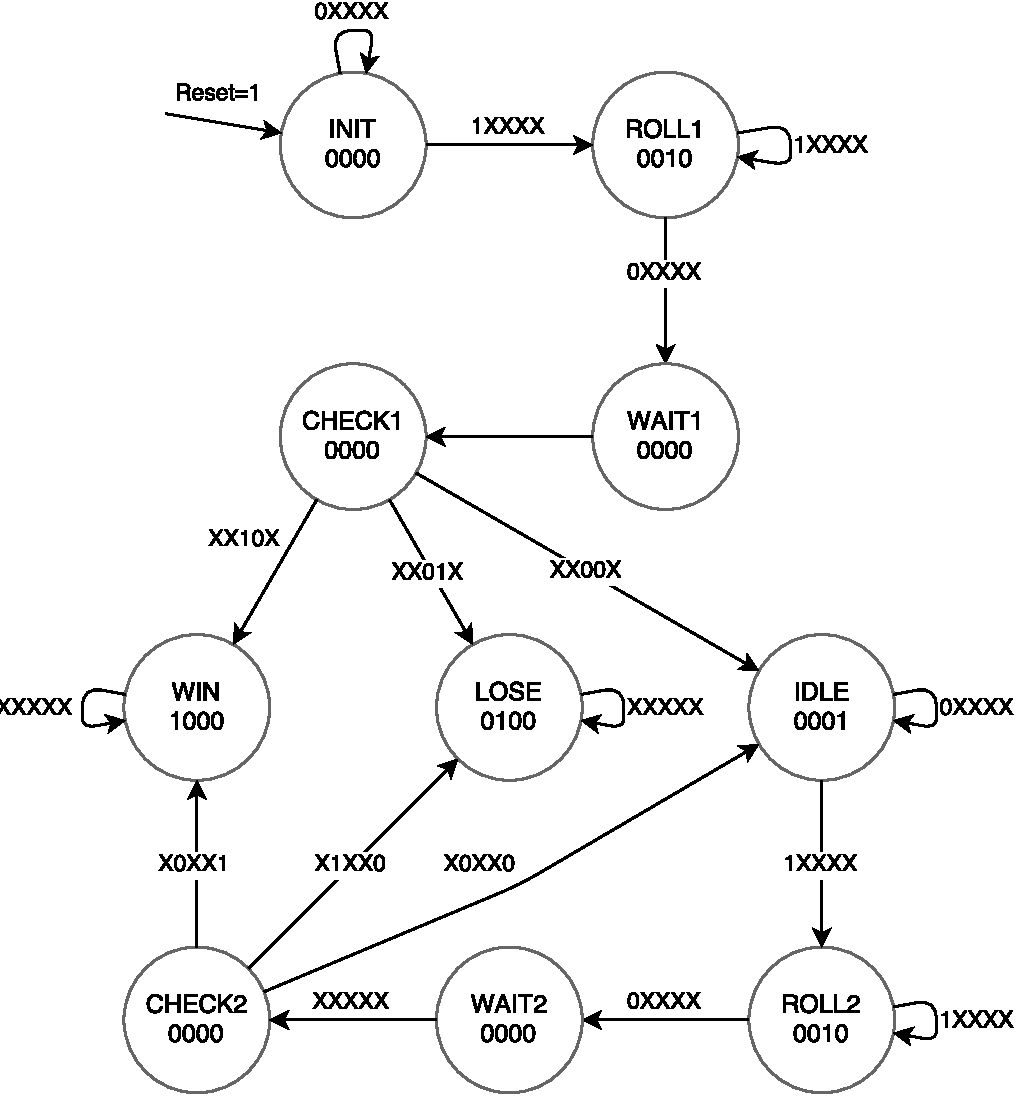
\includegraphics[width=0.6\textwidth]{diagrams/diceGameDiagram.pdf}
\caption{Diagram maszyny stanów bloku \texttt{Control}. Wejścia: \texttt{Rb}, \texttt{D7}, \texttt{D711}, \texttt{D2312}, \texttt{Eq} oraz \texttt{Reset}, wyjścia: \texttt{Win}, \texttt{Lose}, \texttt{Roll}, \texttt{Sp}.}
\label{diceGameDiagram}
\end{figure}




\subsection{Testbench i wyniki symulacji}

Do sprawdzenia poprawności działania został dodany blok \texttt{Game Test}. Diagram maszyny stanów tego bloku został przedstawiony na rys.~\ref{gameTestDiagram}.

\begin{figure}[h]
\centering
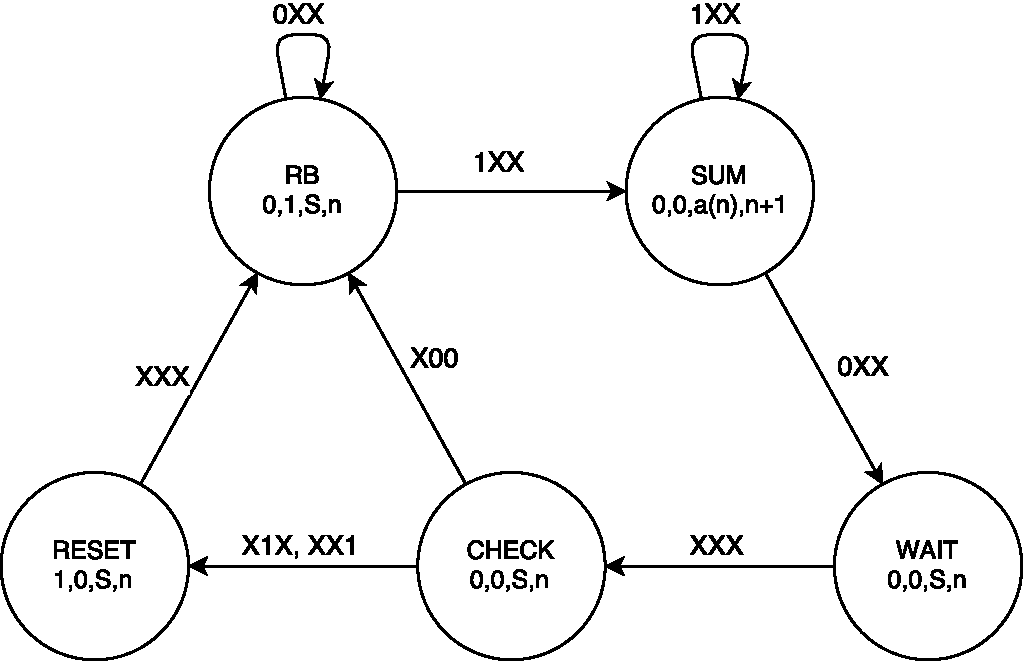
\includegraphics[width=0.5\textwidth]{diagrams/gameTestDiagram.pdf}
\caption{Diagram maszyny stanów bloku \texttt{Game Test}. Wejścia: \texttt{Roll}, \texttt{Win}, \texttt{Lose}, wyjścia: \texttt{Reset}, \texttt{Rb}, \texttt{Sum}. \texttt{n}}
\label{gameTestDiagram}
\end{figure}

Na początku układ znajduje się w stanie \texttt{RB} (w tym stanie symulowane jest naciśnięcie przycisku Roll Button) i przechodzi do stanu \texttt{SUM} po otrzymaniu sygnału \texttt{Roll} równego 1. Stan \texttt{SUM} odpowiada za pobranie $n$--tego elementu z przygotowanej wcześniej tablicy i przypisanie $n=n+1$. Po otrzymaniu sygnału \texttt{Roll} równego 0 układ przechodzi do stanu \texttt{WAIT}, gdzie czeka na otrzymanie poprawnych wyników z bloku \texttt{DG\_NoSum}. Następnie przechodzi do stanu \texttt{CHECK}, a kolejne przejście zależy od sygnałów \texttt{WIN} i \texttt{LOSE}. Jeżeli którykolwiek z nich będzie równy 1, to układ przejdzie do stanu \texttt{RESET}, aby móc ustawić sygnał \texttt{Reset} na 1. W przeciwnym wypadku reset nie jest konieczny, więc układ przechodzi do stanu \texttt{RB}.

Poniżej przestawiono wyniki symulacji przeprowadzonej w programie \textit{Modelsim}. Rys.~\ref{tb_dg_0_1} przedstawia widok na całość przebiegów, a rys.~\ref{tb_dg_0_2} przybliża kilka pierwszych przebiegów.

\begin{figure}[h]
\centering
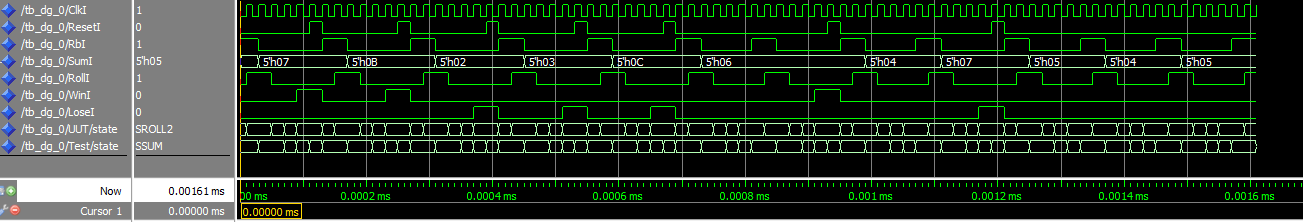
\includegraphics[scale = 0.35]{screens/tb_dg_0_1.png}
\caption{Symulacja układu bez liczników i sumatora -- widok na całość}
\label{tb_dg_0_1}
\end{figure}

Widać, że sumy i odpowiadające im reakcje bloku \texttt{DG\_NoSum} były zgodne z założeniami. W pierwszym cyklu po resecie i ustawieniu sumy na 7 (sytuacja: wygrana), więc układ ustawił sygnał \texttt{WinI} na 1. Kolejny cykl to reset i ustawienie sumy na 11. Również nastąpiła wygrana i ustawienie \texttt{WinI} na 1. Następnie były testowane przegrane. W kolejnych trzech cyklach sprawdzono 3 przypadki wartości sumy: 2, 3 i 12. Wtedy następowało rozpoznanie przegranej i ustawienie sygnału \texttt{LoseI} na 1. Następnie przetestowano wygraną poprzez wylosowanie 2 razy pod rząd tej samej sumy -- zgodnie z oczekiwaniami otrzymano \texttt{WinI} równe 1. Kolejny cykl to suma równa 4, więc układ pozwolił na następne losowanie w ramach tej samej gry. Po wylosowaniu sumy równej 7 nastąpiła przegrana (sygnał \texttt{LoseI} równy 1). Ostatnie cykle pokazują, że jeżeli nie nastąpi ani przegrana, ani wygrana, to można wykonywać kolejne losowania w ramach tej samej gry.


\begin{figure}[h]
\centering
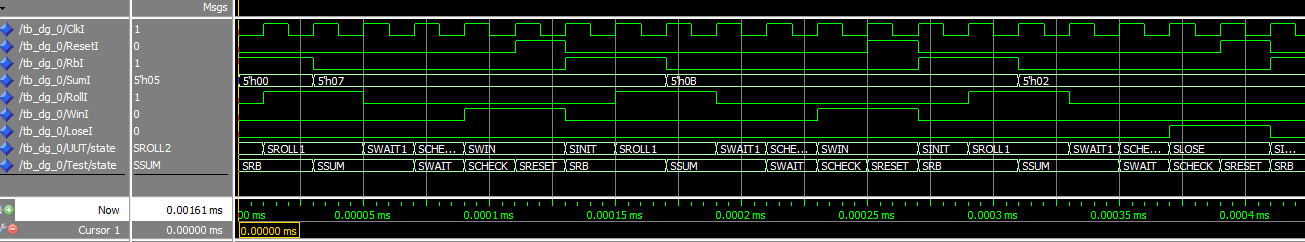
\includegraphics[scale = 0.35]{screens/tb_dg_0_2.png}
\caption{Symulacja układu bez liczników i sumatora -- widok na pierwszy cykl}
\label{tb_dg_0_2}
\end{figure}

Do sprawdzenia poprawności działania maszyn stanów blocków \texttt{DG\_NoSum} i \texttt{Game Test} przybliżono przebiegi. Widać, że zachodzą one zgodnie z założeniami.

\section{Model kompletny -- z licznikami i sumatorem}

\subsection{Struktura układu}

Na rys.~\ref{diceGameAll} przedstawiona jest struktura, na podstawie której napisano kod w VHDL. 

\begin{figure}[h]
\centering
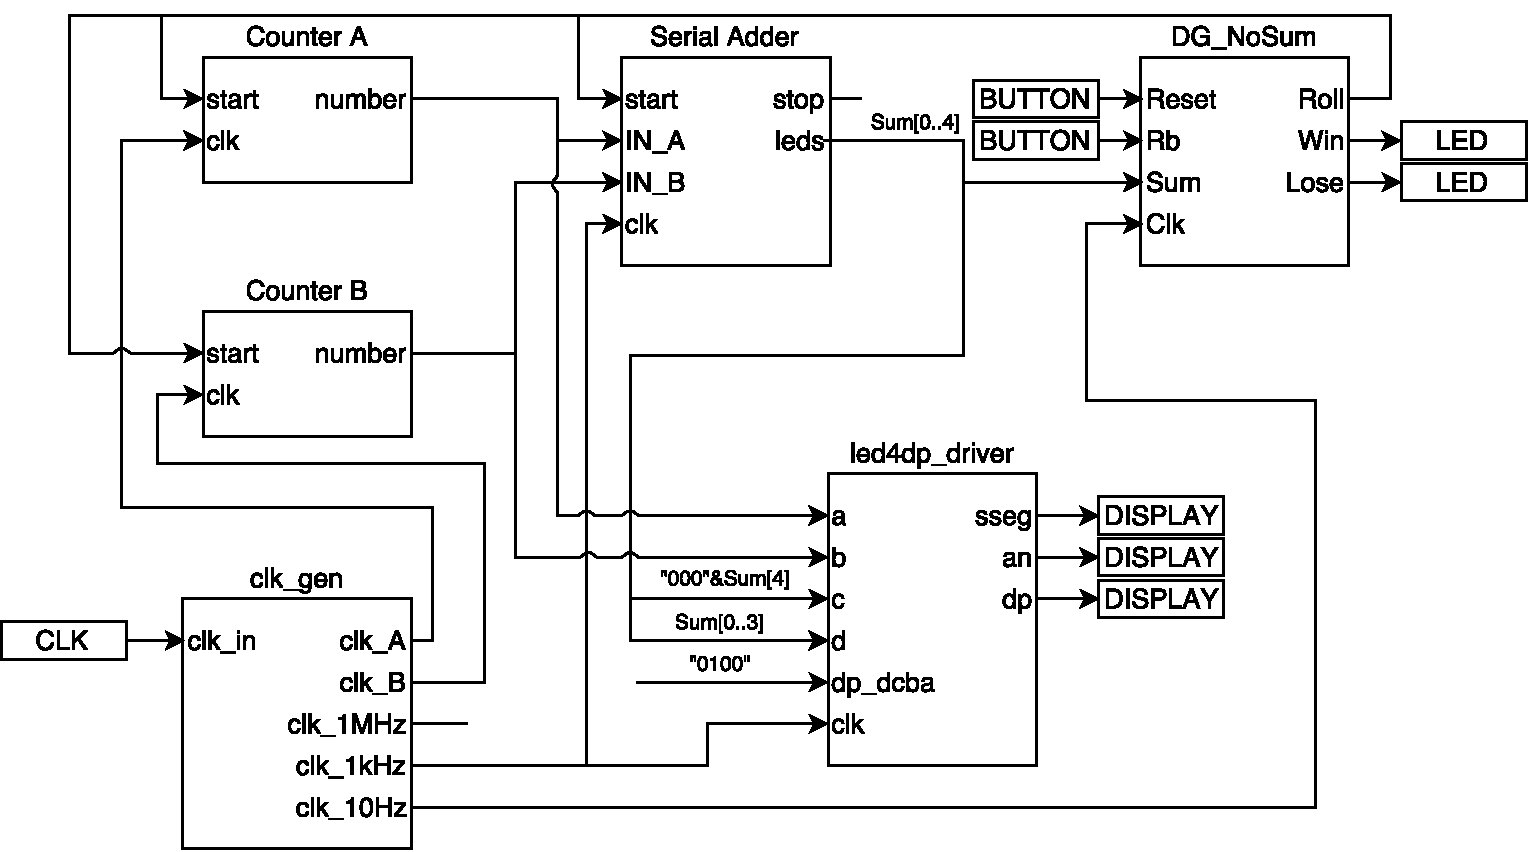
\includegraphics[width=\textwidth]{schematics/diceGameAll.pdf}
\caption{Struktura układu bez liczników i sumatora}
\label{diceGameAll}
\end{figure}

Jest to model dice game z licznikami i sumatorem. Składa się z następujących bloków:
\begin{itemize}
\item \texttt{DG\_NoSum} -- układ dice game bez liczników i sumatora,
\item \texttt{Counter A} i \texttt{Counter B} -- liczniki od 1 do 6, zmieniają wartość, gdy wciśnięty zostanie przycisc Roll Button,
\item \texttt{Serial Adder} -- sumator szeregowy przygotowany na poprzednich zajęciach,
\item \texttt{clk\_gen} -- układ generujący sygnały o różnych częstotliwościach,
\item \texttt{led4dp\_driver} -- układ umożliwiający przedstawienie wyników na wyświetlaczu.
\end{itemize}

Ponadto do sygnałów wejściowych i wyjściowych układy dodano atrybut \texttt{LOC}, aby móc zaimplementować układ na płycie Nexys. Z rys.~\ref{diceGameAll} widać, że sygnał zegarowy zostanie podpięty pod \texttt{clk\_in} (CLK), sygnały \texttt{Win} i \texttt{Lose} zostaną przedstawione na diodach (LED), sygnały \texttt{Reset} i \texttt{Rb} to przyciski (BUTTON), a \texttt{sseg}, \texttt{an} i \texttt{dp} umożliwią odpowietnie ustawienie wyświetlacza (DISPLAY).


Do zasymulowania losowości otrzymywanej sumy do bloków \texttt{Counter A} i \texttt{Counter B} podpięto sygnały zegarowe o różnych częstotliwościach. Inne bloki korzystają jeszcze z innych częstotliwośc, zatem niezbędne było napisanie bloku \texttt{clk\_gen}. Ten blok z sygnału wejściowego o częstotliwości 50 MHz generuje sygnały o potrzebnych częstotliwościach.

\subsection{Testbench i wyniki symulacji}

Do sprawdzenia poprawności działania układu w pliku testbench została zaimpementowana maszyna stanów, której diagram został przedstawiony na rys.~\ref{testbenchAllDiagram}.

\begin{figure}[h!]
\centering
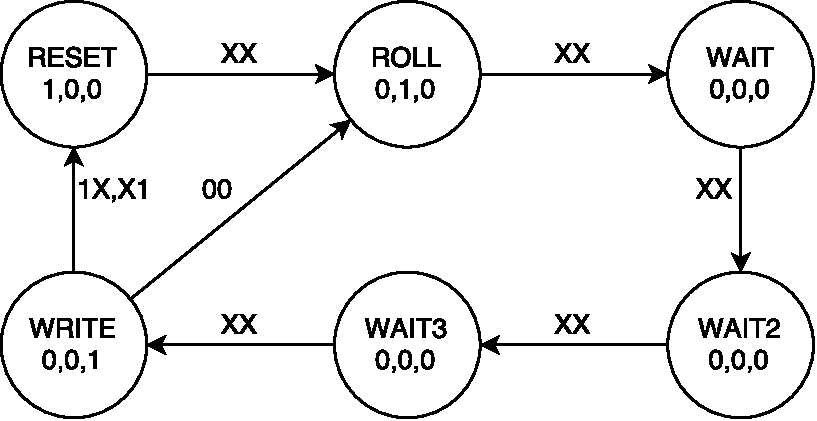
\includegraphics[width=0.5\textwidth]{diagrams/testbenchAllDiagram.pdf}
\caption{Diagram maszyny stanów testbenchu. Wejścia: \texttt{Win}, \texttt{Lose}, wyjścia: \texttt{Reset}, \texttt{Rb}, \texttt{write\_enable}}
\label{testbenchAllDiagram}
\end{figure}

Stanem początkowym jest stan \texttt{RESET}. Wtedy ustawienie sygnału \texttt{Reset} na 1 spowoduje rozpoczęcie nowej gry. Następnie układ przejdzie do stanu \texttt{ROLL}, gdzie zostanie ustawiony na 1 sygnał \texttt{Rb}. Następne 3 stany \texttt{WAIT}, \texttt{WAIT2} i \texttt{WAIT3} nic nie ustawiają, ale są niezbędne do poczekania na poprawne wyniki z układu dice game. Ze stanu \texttt{WAIT3} testbench przechodzi do stanu \texttt{WRITE}. Tam ustawiany jest sygnał \texttt{write\_enable} inicjujący zapis do pliku \texttt{testbench\_results.txt}. Następnie układ przechodzi do stanu \texttt{RESET} jeżeli wykryto przegraną lub wygraną. W przeciwnym wypadku przechodzi do stanu \texttt{ROLL}. 

Poniżej przestawiono wyniki symulacji przeprowadzonej w programie \textit{Modelsim}. Rys.~\ref{pierwsza_gra}--\ref{piata_gra} przedstawiają przebiegi otrzymane podczas symulacji.

\begin{figure}[h]
\centering
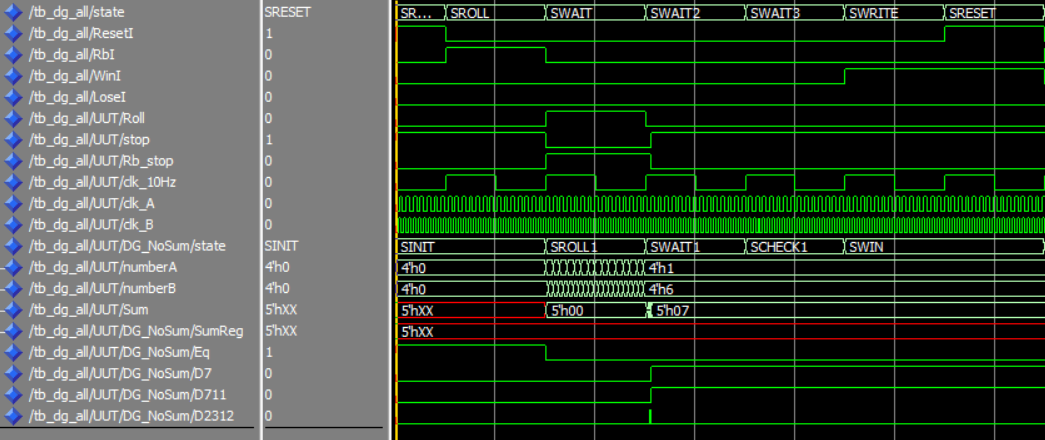
\includegraphics[scale = 0.5]{screens/pierwsza_gra.png}
\caption{Symulacja układu z licznikami i sumatorem -- pierwsza gra}
\label{pierwsza_gra}
\end{figure}

Na powyższym zrzucie ekranu (rys.~\ref{pierwsza_gra}) widać przebiegi dotyczące rozpoczęcia gry i pierwszego rzutu kośćmi. Rzut poprzedzony jest stanem wysokim na sygnale \texttt{ResetI} -- układ jest w tym czasie resetowany, a maszyna stanów gry znajduje się w stanie \texttt{INIT}. Następnie wykonywany jest pierwszy rzut -- sygnał \texttt{Roll} jest w stanie wysokim, sygnał \texttt{stop} przechodzi w stan niski(czyli nieaktywny), a maszyna stanów gry znajduje się w stanie \texttt{ROLL1}. Można zaobserwować, że w tym czasie z różną częstotliwością zmieniają się wartości sygnałów \texttt{numberA} i \texttt{numberB}, które zależą od przebiegów zegarów \texttt{clk\_A} i \texttt{clk\_C}. W ten sposób losowany jest wynik rzutu obu kości. Po puszczeniu przycisku Roll Button układ przechodzi w stan \texttt{WAIT1}, w którym wartości \texttt{numberA} i \texttt{numberB} są już ustalone i wynoszą odpowiednio 1 i 6. Suma, która przechowywana jest w rejestrze \texttt{Sum}, wynosi 7, więc sygnały \texttt{D7} oraz \texttt{D711} są w stanie wysokim. W stanie \texttt{CHECK1} następuje sprawdzenie rezultatu. Ze względu na to, że jest to pierwszy rzut w grze, wylosowanie sumy 7 oznacza wygraną i przejście do stanu \texttt{WIN}. Wówczas nie ma możliwości dalszego ,,rzucania'' kośćmi -- trzeba wykonać reset, aby rozpocząć grę od nowa. 
Warto tu również zwrócić uwagę na stany w testbenchu. Jak widać wyprzedzają one stany układu odpowiadającego za grę. Wcześniej omówiony stan \texttt{RESET} odpowiada za wyzerowanie układu, \texttt{ROLL za rzucenie kośćmi}, \texttt{WAIT}, \texttt{WAIT2}, \texttt{WAIT3} odpowiadają za oczekiwanie na wynik, a \texttt{WRITE} za zapis wyniku do pliku tekstowego.

Ze względu na fakt, iż powyżej zostały omówione wszystkie najważniejsze elementy testbenchu, tj. stany i omówienie znaczenia wartości poszczególnych sygnałów, dla kolejnych gier zostaną omówione tylko najistotniejsze różnice.

\begin{figure}[h]
\centering
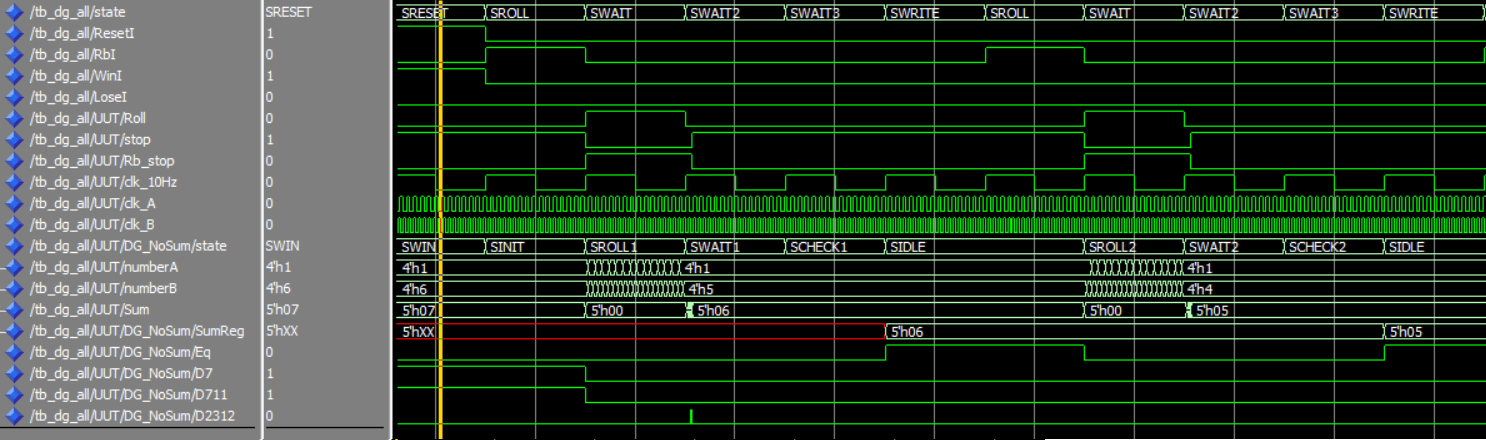
\includegraphics[scale = 0.5]{screens/druga_gra_1.png}
\caption{Symulacja układu z licznikami i sumatorem -- druga gra}
\label{druga_gra_1}
\end{figure}

Zamieszczony kolejny zrzut ekranu (rys.~\ref{druga_gra_1}) prezentuje rozpoczęcie drugiej gry i wykonanie dwóch rzutów kośćmi. Po pierwszym rzucie otrzymano wyniki dla \texttt{numberA} oraz \texttt{numberB} odpowiednio 1 i 5, co w sumie daje 6. Oznacza to konieczność wykonania kolejnego rzutu. W kolejnym rzucie otrzymujemy wartości 1 i 4, co w sumie daje 5 i również nie pozwala stwierdzić, czy rozgrywka zakończyła się zwycięstwem czy porażką. 

\begin{figure}[h]
\centering
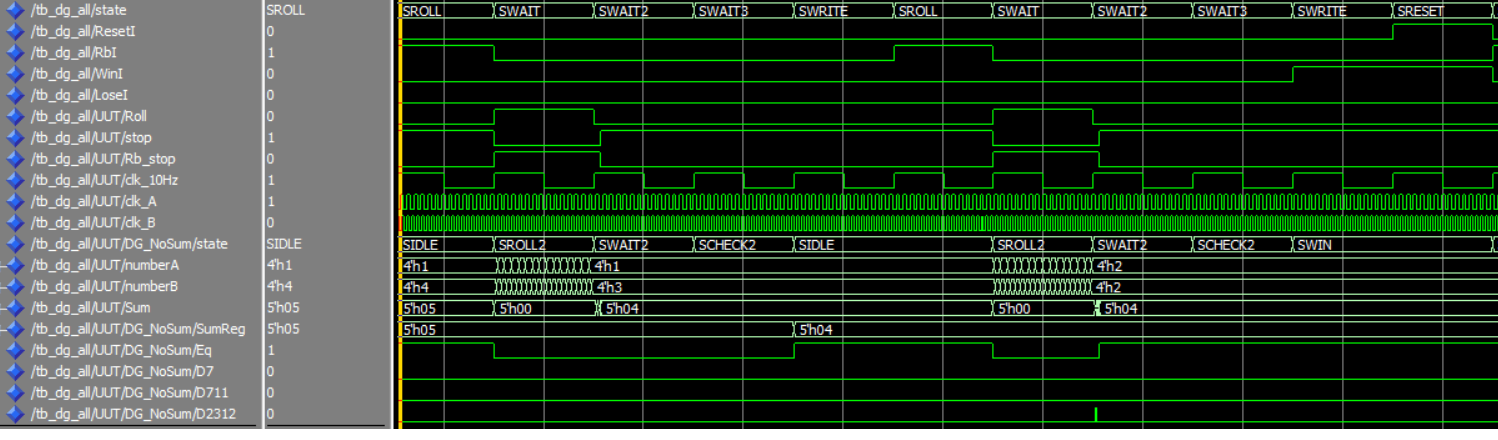
\includegraphics[scale = 0.5]{screens/druga_gra_2_win.png}
\caption{Symulacja układu z licznikami i sumatorem -- druga gra, kolejne rzuty}
\label{druga_gra_2}
\end{figure}

Wykonywany jest zatem kolejny rzut (rys.~\ref{druga_gra_2}). On również nie pozwala na określenie statusu gry, bowiem wylosowane wartości to 1 i 3, w sumie 4. Dopiero ostatnia kolejka przynosi oczekiwany rezultat, ponieważ wyrzucone zostają wartości 2 i 2, w sumie 4 -- bieżąca suma jest równa poprzedniej, oznacza to zatem wygraną.

\begin{figure}[h]
\centering
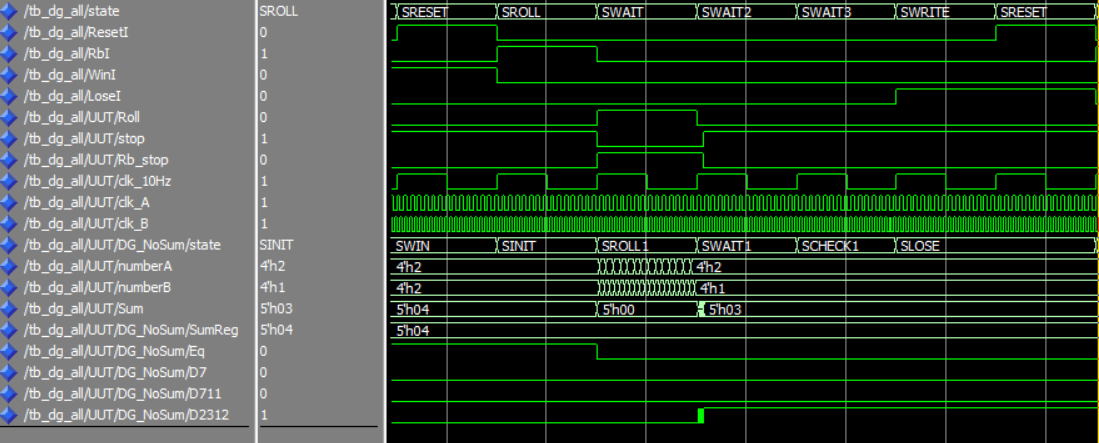
\includegraphics[scale = 0.5]{screens/trzecia_gra.png}
\caption{Symulacja układu z licznikami i sumatorem -- trzecia gra}
\label{trzecia_gra}
\end{figure}

Zamieszczony następny zrzut (rys.~\ref{trzecia_gra}) obrazuje trzecią grę wykonaną w ramach testbenchu. W tym przypadku w pierwszym rzucie wypadają wartości 2 i 1, czyli w sumie 3, co oznacza przegraną.

\begin{figure}[h]
\centering
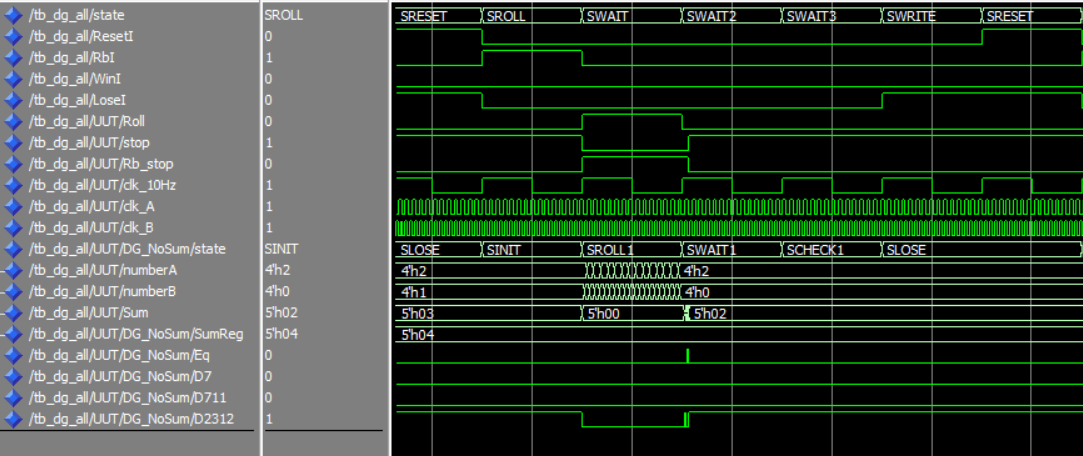
\includegraphics[scale = 0.5]{screens/czwarta_gra.png}
\caption{Symulacja układu z licznikami i sumatorem -- czwarta gra}
\label{czwarta_gra}
\end{figure}

W czwartej grze (rys.~\ref{czwarta_gra}), podobnie jak w trzeciej, również wynikiem jest przegrana. W pierwszym rzucie wypadają wartości 2 i 0, czyli łącznie 2. Taka suma po pierwszym rzucie oznacza przegraną, zgodnie z regułami gry.

\begin{figure}[h]
\centering
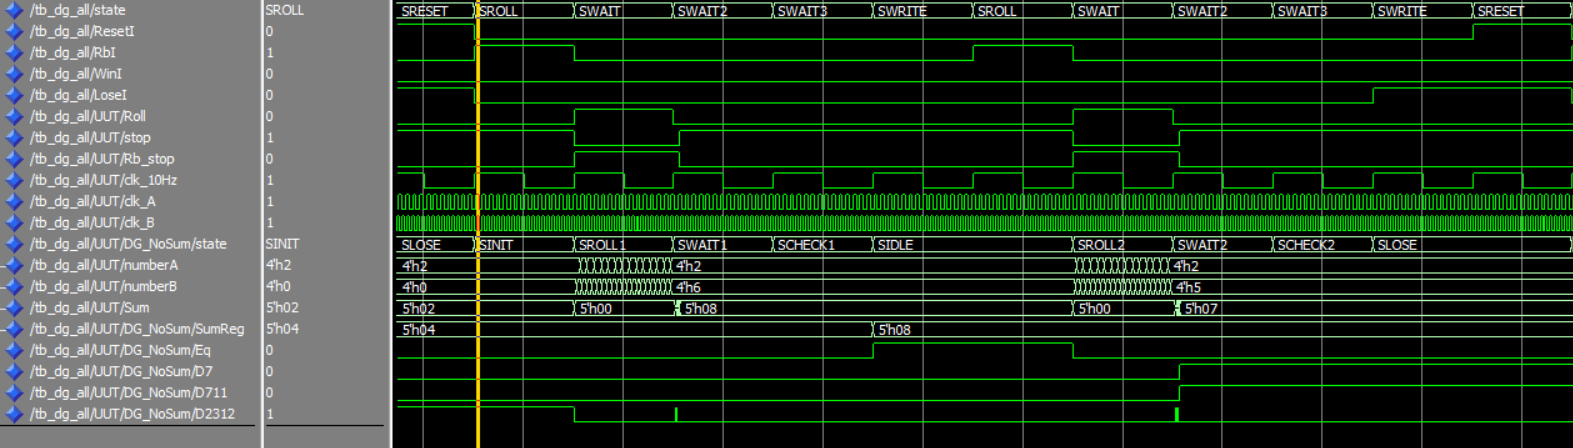
\includegraphics[scale = 0.5]{screens/piata_gra.png}
\caption{Symulacja układu z licznikami i sumatorem -- piąta gra}
\label{piata_gra}
\end{figure}

Piąta gra (rys.~\ref{piata_gra}) także przedstawia przypadek przegranej, ale wynikającej z faktu, iż w drugim rzucie suma wylosowanych wartości była równa 7.


Wyniki symulacji zostają także zapisane do pliku tekstowego. Zawartość takiego pliku została przedstawiony w listingu~\ref{lst:tr}. Struktura pliku składa się z następujących kolumn:
\begin{itemize}
\item \texttt{Time} -- czas, w którym nastąpił zapis do pliku,
\item \texttt{A} -- wartość wyjścia z pierwszego licznika,
\item \texttt{B} -- wartość wyjścia z drugiego licznika,
\item \texttt{SUM} -- wartość wyjścia z sumatora,
\item \texttt{Win} -- wartość sygnału \texttt{WinI},
\item \texttt{Lose} -- wartość sygnały \texttt{LoseI},
\item \texttt{Game} -- opis mówiący, czy dana gra jest rozpoczynana (\texttt{NEW}), czy następuje kolejne losowanie w rammach tej samej gry (wtedy w kolumnie jest puste pole).
\end{itemize}

\lstinputlisting[style=VHDLStyle,label=lst:tr,caption={Zawartość pliku \texttt{testbench\_results.txt} -- wyniki symulacji}]{testbench_results.txt}

Z listingu widać, że nastąpiło 10 rzutów kośćmi. Widać również, że pierwsze losowanie zakończyło się wygraną, więc kolejne losowanie jest rozpoczęciem nowej gry. Ta gra również kończy się wygraną -- wygrana poprzez wylosowanie dwóch takich samych sum pod rząd. Następna nowa gra jest zapisana w linii 7 i kończy się ona przegraną (wylosowanie sumy 3). Podobna sytuacja jest w linii 8 -- przegrana poprzez wylosowanie sumy 2. Kolejne 2 linie przedstawiają kolejną grę -- widać, że została ona przegrana przez otrzymanie sumy równej 7 przy drugim rzucie. Ostatni rzut nie zakończył się ani porażką, ani wygraną, zatem kolejne losowanie nastąpiłoby w ramach tej samej gry.

\subsection{Nexys}

Przypisano odpowiednie piny płytki Nexys do sygnałów:
\begin{itemize}
\item \texttt{Clk} -- B8,
\item \texttt{Reset} -- B18,
\item \texttt{Rb} -- D18,
\item \texttt{Win} -- J14,
\item \texttt{Lose} -- J15,
\item \texttt{sseg} -- H14, J17, G14, D16, D17, F18, L18,
\item \texttt{an} -- F17, H17, C18, F15,
\item \texttt{dp} -- C17.
\end{itemize}

W środowisku \textit{ISE Xilinx} stworzono projekt, dokonano syntezy i wygenerowano plik \texttt{.bit}. Żadne błędy nie zostały wykryte podczas tych procesów. 
Po uruchomieniu programu na płytce Nexys wykonano testy działania. Nie wykryto zachowań niezgodnych z założeniami.

\section{Wnioski}

Zrealizowany projekt pozwolił studentom na utrwalenie swoich umiejętności z implementacji maszyn stanu w VHDL. Ponadto zapoznano się z tworzeniem projektu syntezowalnego, aby móc wgrać go na płytkę Nexys. Symulacja w programie \textit{Modelsim} i działanie układu na płycie Nexys przebiegło zgodnie z założeniami projektu.



\end{document}






